\section{Bode-Diagramm}

Das Bode-Diagramm ist eine weitere Variante, den Frequenzgang $G(\jimg \omega)$ grafisch darzustellen.
Die Darstellung beinhaltet zwei Graphen.

\begin{itemize}
    \item Amplitudengang $|G(\jimg \omega)|$ in Dezibel $\deci \bel$
    \item Phasengang $\angle G(\jimg \omega)$ in Grad $\degree$
    \item Die Frequenzachse ist \textbf{logarithmisch} mit $\log_{10}(\omega)$
    \item \textbf{Ein Bodediagramm kann in ein Nyquistdiagramm umgezeichnet werden, aber nicht umgekehrt!}
\end{itemize}


% Bei zu wenig Platz weglassen
\subsubsection{Logarithmische Frequenzachse}

\begin{outline}
    \1 Serieschaltung von Systemen
        $$ G(\jimg \omega) = G_1(\jimg \omega) \cdot G_2(\jimg \omega) $$

        \2 Amplitudengang
            $$ |G(\jimg \omega)| = |G_1(\jimg \omega)| \cdot |G_2(\jimg \omega)| $$
            $$ |G(\jimg \omega)|_{\deci \bel} = |G_1(\jimg \omega)|_{\deci \bel} + |G_2(\jimg \omega)|_{\deci \bel} $$
            \textrightarrow\ Grafisch multiplizieren wäre schwierig, grafisch addieren geht gut

        \2 Phasengang
            $$ \angle G(\jimg \omega) = \angle G_1(\jimg \omega) +  \angle G_2(\jimg \omega) $$
            \textrightarrow\ Die Phase muss nicht logarithmisch sein, wir haben schon eine Addition 
\end{outline}


\subsection{Vorgehen: Bode-Diagramm zeichnen}

Das Diagramm wird approximativ mit \textbf{Geraden} gezeichnet!

\begin{outline}
    \1 Frequenzgang in folgende Form bringen:
        $$ G(\jimg \omega) = K_0 \cdot (\jimg \omega)^v \cdot \frac{(1 + T_{n0} \cdot \jimg \omega)\cdot (1 + T_{n1} \cdot \jimg \omega) \cdot \ldots}
        {(1 + T_{p0} \cdot \jimg \omega)\cdot (1 + T_{p1} \cdot \jimg \omega) \cdot \ldots} \cdot e^{- \jimg \omega T_t} $$
        \2 Für $\omega = 0$ sind alle $(1 + T \cdot \jimg \omega) = 1 = 0 \, \deci \bel$
        \2 Für $\omega = \frac{1}{T}$ sind alle  $(1 + T \cdot \jimg \omega) = 1 + \jimg = \sqrt{2} \cdot e^{\jimg \frac{\pi}{4}} 
            = 3 \, \deci \bel \angle 45 \, \degree$
    \1 Frequenzen der Nullstellen berechnen: $\omega = \frac{1}{T_n}$
    \1 Frequenzen der Polstellen berechnen: $\omega = \frac{1}{T_p}$


    \1 Jede \textbf{Nullstelle} bewirkt
        \2 einen Knick um $+ 20 \deci \bel$ / Dekade \textbf{nach oben} im Amplitudengang
        \2 einen Phasenhub von $+ 90 \, \degree$ über 2 Dekaden \textrightarrow\ $+ 45 \, \degree$ beim Knick
    \1 Jede \textbf{Polstelle} bewirkt
        \2 einen Knick um $- 20 \deci \bel$ / Dekade \textbf{nach unten} im Amplitudengang
        \2 einen Phasenverlust von $- 90 \, \degree$ über 2 Dekaden \textrightarrow\ $- 45 \, \degree$ beim Knick
    \1 Einzelne Faktoren einzeichnen \textrightarrow\ Wenn Faktor quadriert ist, zwei mal einzeichnen!
    \1 Grafische Addition der Faktoren für gesamten Frequenzgang
\end{outline}


\example{Bode-Diagramm zeichnen}
\vspace{-0.2cm}
$$ G(\jimg \omega) = \frac{\jimg \omega + 10}{(\jimg \omega + 0.1)} \quad  \underrightarrow{\text{ Standardform }} \quad 
  G(\jimg \omega) = \cgn{100} \cdot \frac{(\cvt{1 + 0.1 \, \jimg \omega})}{(\cbl{ 1 + 10 \, \jimg \omega})} $$

  \begin{itemize}
    \item $ \cgn{\abs{K_0}_{\deci \bel} = \abs{100}_{\deci \bel} = 40 \, \deci \bel}$ \textrightarrow\ $\angle G(100) = 0 \, \degree$
    \item Nullstelle: \cvt{$\abs{1 + 0.1 \, \jimg \omega}_{\deci \bel}$} \textrightarrow\ Knick bei $\omega = \frac{1}{0.1 \second} = 10 \frac{\rad}{\second}$
    \item Polstelle: \cbl{$\abs{1 + 10 \, \jimg \omega}_{\deci \bel}$} \textrightarrow\ Knick bei $\omega = \frac{1}{10 \second} = 0.1 \frac{\rad}{\second}$
    \item \cor{Endresultat}: Grafische Addition der Teilresultate
  \end{itemize}

\begin{center}
    % Gain
    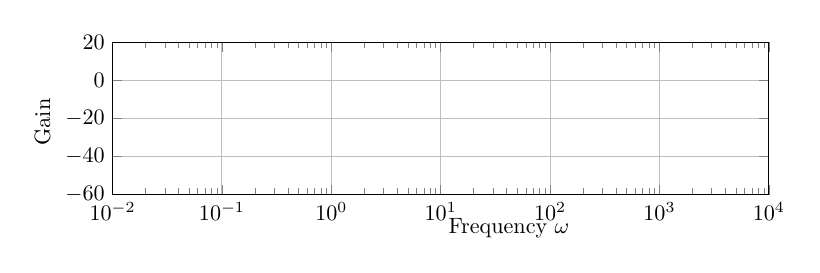
\begin{tikzpicture}
        [
            scale = 0.8,
            >=latex
        ]
        \begin{axis}
            [
                width=12cm,
                height=4cm,
                xmode=log,
                xmin=0.01, xmax=10000, ymin=-60, ymax=20,
                x label style={anchor=west},
                xlabel=Frequency $\omega$,
                y label style={anchor=south},
                ylabel=Gain $\deci \bel$,
                grid
            ]
            
            % coordinates
            
            % draw connections

            
           
        \end{axis}
        
    \end{tikzpicture}

    \vspace{0.3cm}


    % Phase
    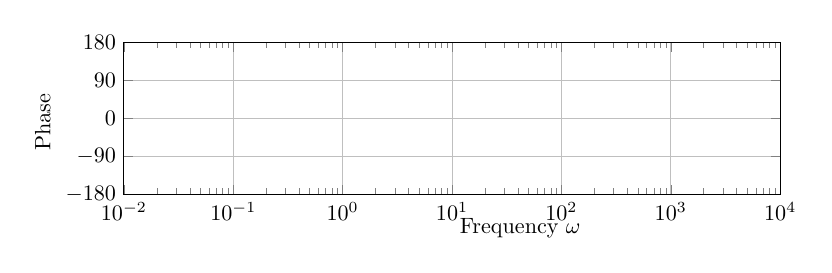
\begin{tikzpicture}
        [
            scale = 0.8,
            >=latex
        ]
        \begin{axis}
            [
                width=12cm,
                height=4cm,
                xmode=log,
                xmin=0.01, xmax=10000, ymin=-180, ymax=180,
                x label style={anchor=west},
                xlabel=Frequency $\omega$,
                y label style={anchor=south},
                ylabel=Phase $\degree$,
                ytick={-180, -90, 0, 90, 180},
                % yticklabels={-180, -90, 0, 90, 180},
                grid
            ]
            
            % coordinates
            
            % draw connections

            
            
        \end{axis}
            
    \end{tikzpicture}
\end{center}


\subsubsection{Inverse Frequenzgänge}

Das Bodediagramm des inversen Frequenzgangs $\frac{1}{G(\jimg \omega)}$ entspricht dem an der $0 \, \deci \bel$-Achse 
\textbf{gespiegelten} Bodediagramm des Frequenzgangs $G(\jimg \omega)$ 
\vspace{0.2cm}
 
\includegraphics[width=\columnwidth]{images/inverse_frequenzgaenge.png}


% Freestyle by Simi, (noch) nicht in Vorlesung behandelt
\subsection{Stabilität im Bodediagramm}
Analog zum Punkt $-1$ im Nyquistdiagramm kann die Stabilität auch im Bodediagramm beurteilt werden.

\begin{itemize}
    \item \textbf{Grenzstabilität}: Amplitudengang bei $0 \, \deci \bel$ \textbf{und} Phasengang bei $-180 \, \degree$
    \item \textbf{Instabilität}: Amplitudengang $>0 \, \deci \bel$
    \item \textbf{Stabilität}: Amplitudengang $<0 \, \deci \bel$
\end{itemize}


% Freestyle by Simi, (noch) nicht in Vorlesung behandelt
\subsubsection{Stabilitätsreserven}

\begin{itemize}
    \item \textbf{Verstärkungsreserve}: $K_{RES}$ entspricht Verstärkung (Amplitude) bei Phase $-180 \, \degree$
    \item \textbf{Phasensreserve}: $\Phi_{RES}$ entspricht Phase bei Verstärkung (Amplitude) $0 \, \deci \bel$
\end{itemize}